\documentclass[a4paper,11pt]{article}

\usepackage[utf8]{inputenc}
\usepackage[T1]{fontenc}
\usepackage[francais]{babel}
\usepackage{lmodern}
\usepackage{geometry}
\geometry{letterpaper}

\usepackage{doc}
\usepackage{url}

\usepackage{graphicx}
\usepackage{epstopdf}
\usepackage{color}
\DeclareGraphicsRule{.tif}{png}{.png}{`convert #1 `dirname #1`/`basename #1 .tif`.png}


\geometry{hscale=0.85,vscale=0.85,centering}
\title{Protocole}
\author{Jean-Baptiste Dalle - Romain Gaborieau - Kevin Hivert - Alexis Braine}
\date{}

\begin{document}

\maketitle

\clearpage

\tableofcontents

\clearpage

\section*{Introduction}
Dans le cadre du premier semestre du Master 1 Informatique de l'Université d'Angers, nous avons été amenés à réaliser un projet rattaché à deux unités d'enseignement : Génie Logiciel et Réseaux. Le but de ce projet était de réaliser un logiciel permettant de \textbf{dessiner collaborativement}. On entend par là un logiciel permettant à plusieurs utilisateurs de coopérer dans la réalisation d'un dessin.

\paragraph{} Étant rattaché à deux matières, ce projet induit deux aspects importants :

\begin{itemize}
	\item L'aspect Génie Logiciel, regroupant plusieurs procédés tels que l'analyse des besoins, l'estimation du temps requis, la structuration des tâches, le management des différents éléments de l'équipe etc.
	\item L'aspect Réseau, regroupant de manière plus technique l'implémentation d'un protocole visant à faire communiquer plusieurs instances du logiciel, l'architecture réseau utilisée, la sécurité mise en œuvre etc.
\end{itemize}

\paragraph{} Dans le but de fournir une solution convenable et en adéquation avec les consignes du sujet, nous avons suivi une succession d'étapes qui seront expliquées dans ce rapport. Dans un premier temps, nous expliquerons l'analyse effectuée avant le développement de notre application, puis la façon dont nous l'avons développé pour finalement expliquer les méthodes utilisées pour le management et la bonne tenue du projet.


\section*{Problématique}
Tout au long de ce projet, nous avons été confrontés à des choix de méthodes, d'implémentation et de structuration. La problématique est donc :

\textit{Comment réaliser un projet tout en utilisant des méthodes adaptées à sa bonne réalisation ?}


\section{Lancement du projet}
\subsection{Scénario nominal/alternatif}
Définition d'un scénario nominal et alternatif

\paragraph{} Dans le cadre de ce projet et notamment de son analyse, nous avons défini un scénario nominal, expliquant l'utilisation normale du logiciel par des utilisateurs avertis, puis un scénario alternatif, décrivant de quelle façon seront gérés certains cas évident comme la perte de connexion.

Scénario nominal

\begin{itemize}
	\item[1]Le « propriétaire » lance le serveur.
	\item[2]Deux utilisateur A et B se connectent sur le serveur.
	\item[3]A peut donc prendre la main. Il dessine quelques formes.
	\item[4]B demande la main.
	\item[5]Lorsque A perd la main (volontairement ou par inactivité), B récupère la main et peut maintenant dessiner.
	\item[6]A et B peuvent exporter le dessin sur leur machine (au format .jpeg ou .svg).
	\item[7]A et B se déconnectent.
\end{itemize}

Scénario alternatif

\begin{itemize}
	\item[1]Le « propriétaire » lance le serveur
	\item[2]Deux utilisateur A et B se connectent sur le serveur.
	\item[3]A, ayant rejoins en premier le salon, à la main et décide d'importer un dessin au format .svg. Puis il dessine quelques formes.
	\item[4]A perd sa connexion internet.
	\item[5]La main passe automatiquement à B qui est alors le seul utilisateur encore présent dans ce salon.
	\item[6]B peut exporter le dessin sur sa machine.
	\item[7]B se déconnecte.
\end{itemize}

\paragraph{} Bien qu'il existe de nombreux autres cas comme par exemple la succession de demande de prise de main, la perte de connexion de tous les utilisateurs etc. ces deux scénarios résument de manière simple et compréhensible les attentes en terme de fonctionnalités de notre application.


\subsection{Analyse}
Une fois les objectifs fixés, nous avons commencé à réfléchir à ce dont nous aurions besoin pour notre projet ainsi que de la façon dont nous allions le structurer.

\subsubsection{Image}
Dans un premier temps, nous avons réfléchi à la façon de stocker les images qui seront utilisées par notre application. Nous avons opté pour le dessin vectoriel et plus particulièrement pour le svg, format qui permet d'enregistrer un dessin vectoriel en xml. Cette solution permet notamment d'utiliser une syntaxe claire pour représenter le dessin. En effet, chaque forme correspond à une balise et il sera donc aisé de rajouter et/ou modifier des formes.

\paragraph{} Nous avons aussi pensé qu'il serait bon que l'utilisateur puisse exporter son image sous un autre format plus commun comme le jpeg par exemple. 

\subsubsection{Architecture}
Après avoir analysé et débattu sur le sujet, nous avons défini que l'application suivrait l'architecture Client/Serveur. En effet, cette architecture permet de centraliser dans un seul serveur toutes les données nécessaires au(x) client(s). Cette centralisation nous permettra de stocker en un point les images de manière à ce que tous les clients puissent y accéder sans avoir à questionner les autres clients.

\paragraph{} Cette architecture sera couplée, pour le côté Client à une architecture MVC, qui est un design pattern particulièrement adapté à l'élaboration d'application ayant un aspect graphique. Cette architecture sépare le Client en 3 parties : le modèle, qui contient les données de l'application, la vue, qui correspond à l'affichage de l'application et le contrôleur, qui effectue les modifications de la vue et du modèle lorsque l'utilisateur interagit avec la vue. 

\paragraph{} Dans le cas d'un couplage avec une architecture Client/Serveur, le contrôleur agira sur le modèle et la vue comme l'impose l'architecture MVC mais agira aussi sur le serveur en envoyant des messages en fonctions des actions de l'utilisateur sur la vue. A l'inverse, lorsque le serveur communique avec le client, il s'occupera de modifier les données et de mettre à jour la vue en conséquence.

\paragraph{} Finalement, nous avons opté pour le design pattern Singleton pour plusieurs de nos composants. En effet, celui-ci permet de s'assurer que, pour une classe l'implémentant, on ne puisse avoir qu'une seule instance de celle-ci. L'utilisation de ce design pattern nous permet ainsi de s'assurer qu'il n'existera qu'une seule instance des composants graphique et du modèle pour un même client.

\paragraph{} Par exemple, lorsque l'utilisateur ouvrira pour la première fois la fenêtre d'aide, celle-ci sera instanciée et affiché. Si l'utilisateur décide de fermer cette fenêtre puis de la rouvrir plus tard, il s'agira de la même instance car elle a été conservé grâce au Singleton. Cela permet de nous assurer notamment que, chaque fois que l'utilisateur ouvre la fenêtre d'aide, il ne soit pas créer une nouvelle instance de la fenêtre qui ne sera ensuite plus jamais utilisée.

\subsubsection{Normes de développement}
Nous avons aussi mis en avant quelques normes de développement. En premier lieu, nous avons décidé de centraliser les différentes constantes comme les chaînes de caractère utilisées pour les titres, les menu, les messages d'erreur. Ainsi, la modification des texte de l'application est simplifiée par le fait que tous les messages se trouvent au même endroit. Cependant, nous avons aussi du faire attention à n'utiliser les constantes que si leur utilisation concordait. Par exemple, deux boutons peuvent utiliser la chaîne « Valider » mais il faut être certains que leur comportement est le même car en cas de modification, l'application pourrait ne plus être cohérente.

\paragraph{} Ensuite, nous avons décidé de procéder à un découpage strict des fonctions de l'application : Un composant graphique correspond à une classe. Le listener de ce composant correspond à une autre classe et n'est pas interne au composant afin de bien séparer l'aspect Contrôleur de l'aspect Vue. De façon à bien représenter cette séparation, nous avons ordonné nos packages de la façon suivante : 

\begin{itemize}
	\item Un composant graphique se trouvera dans le package \texttt{dessin.collaboratif.view.component}. Cette hiérarchie est poursuivie par le type de composant. Ainsi, le bouton « Quitter » du menu se trouvera dans \texttt{dessin.collaboratif.view.component.menu.item}
	\item Un contrôleur aura toujours la même hiérarchie de package que le composant auquel il est rattaché, à ceci près que le package view est remplacé par le package controller. Pour l'exemple précédent, la classe permettant d'écouter le clic sur le bouton quitter se trouvera dans \texttt{dessin.collaboratif.controller.components.menu.item}
	\item Une classe JUnit permettant de tester les fonctionnalités d'un composants se trouvera de la même façon dans un package test. Toujours pour l'exemple précédent, une possible classe JUnit permettant de tester la fonction quitter se trouvera dans \texttt{dessin.collaboratif.test.components.menu.item}
	\item Les classes correspondant aux données seront situé dans \texttt{dessin.collaboratif.model}, néanmoins, les données étant communes à tous les composants, la suite de la hiérarchie est différentes des composants qui l'utilisent.
	\item La classe GeneralVariables contenant toutes les constantes ainsi que les différentes énumération se trouveront dans \texttt{dessin.collaboratif.misc}
\end{itemize}

\paragraph{} Finalement, alors que l’arborescence de \texttt{dessin.collaboratif} correspond au client, le package \texttt{server} correspond au server. Le dernier package \texttt{launcher} est le lien entre les deux packages précédent et fournit des classes permettant de lancer le client, le serveur ou les deux.

\paragraph{} Bien que cette hiérarchie puisse sembler laborieuse, elle permet très facilement de comprendre la fonction de la classe en question par rapport à l'endroit où elle se situe et l'affichage hiérarchique que fournit la plupart des IDE comme Eclipse permet de s'y déplacer facilement.

\subsubsection{UML}
Afin de donner un cadre au projet, nous avons mis en place un UML pour représenter la hiérarchie des classes ainsi que leur utilisation entre elles. Grâce à la hiérarchie des packages expliqué plus tôt, il fut très simple d'organiser ses classes entre elles tout en faisant un découpage clair des fonctionnalités. 

\paragraph{} Dans le but d'avoir un UML lisible, nous avons préféré créer une version simplifié de celui-ci. En effet, plutôt que d'afficher toutes les classes liées à l'interface graphique, nous avons inséré le package view. De la même manière, pour le controlleur, nous n'avons inséré que le package.

\paragraph{} Ainsi, notre UML permet de comprendre les interactions entre les différents composants du projet, représenté soit par des packages, soit par des classes.

\subsubsection{Chiffrage}
Le chiffrage correspond à la partie de l'analyse durant laquelle il a fallu déterminer le temps que prendrait les différentes tâches afin de pouvoir les organiser pour réaliser le planning. La difficulté de cette étape fut en premier lieu de trouver un temps de développement cohérent pour les différentes tâches. En règle générale, une entreprise demandera à quelqu'un ayant l'habitude de réaliser ce genre de chiffrage et qui notamment possède une bonne expertise technique afin de chiffrer de manière cohérente. Dans notre cas, bien que nous puissions estimer la charge demandée, il est difficile de toujours donner un chiffrage cohérent. De plus, étant donné que la réalisation de ce projet s'est fait en parallèle d'autres projets et cours, aucun de nous ne pouvait être réellement compt\'e comme une ressource à part entière.

\paragraph{} Cette situation ressemble beaucoup à des situations similaires connues en entreprise comme lorsque l'équipe comprend un alternant ou bien un développeur travaillant sur plusieurs projets et n'étant pas disponible tous les jours.

\paragraph{} Notre chiffrage a donc été réalisé en prenant en compte ces différents points. Au fur et à mesure des développements, nous nous sommes rendu compte que certaines tâches avaient été sur-chiffrées et que, bien qu'elles semblaient complexes, une fois l'environnement technique appréhendé, elles se révélèrent plus simples que prévue. A l'inverse, certaines tâches que nous pensions aisées à réaliser se sont révélées plus ardues que prévu ou ont mis à jour certaines difficultés que nous n'avions pas prise en compte.

\paragraph{} En considérant l'avance prise sur certaines tâches et le retard pris sur d'autre, nous avons dans l'ensemble plutôt bien respecté les délais, ce qui nous a laissé une bonne marge de manœuvre pour la rédaction du rapport et la recette. De manière à ne pas mettre en péril le projet, nous avons pensé à certaines fonctionnalités non demandées dans le sujet que nous avons qualifié de facultatives et n'en avons réalisé que certaines. Néanmoins, sans cette phase d'analyse, nous aurions peut-être perdu trop de temps pour des éléments non présent dans le cahier des charges, ce qui n'est pas admissible car le respect des délais est un point capital, que ce soit pour ce projet ou en entreprise.

\subsection{Choix de solution}
Dans le cadre de notre projet, nous avons été amenés à choisir un certain nombre de solutions afin de répondre le mieux possible au cahier des charges. Les solutions à choisir peuvent être distinguées en deux types : les bibliothèque de développement, qui nous ont permises de développer certaines parties du projet, et qui sont donc liées au langage utilisé (ici Java) et les outils de développement, qui ont permis de simplifier certains process de la gestion de projet, notamment le versionning, le planning etc.

\subsubsection{Bibliothèque}
Dans un premier temps, notre application disposant d'une interface graphique, nous devions choisir la bibliothèque graphique que à utiliser. En Java, il existe plusieurs bibliothèque graphique. Nous avons sélectionné deux bibliothèques : Swing et JavaFX.

\paragraph{} Swing est la bibliothèque graphique la plus connue. Elle est basée sur une autre bibliothèque nommée AWT. Bien qu'elle soit moins efficace qu'AWT, Swing facilite la création d'interface et fournit notamment une interface qui ne varie pas suivant le système d'exploitation utilisé. Finalement, il favorise l'utilisation du design pattern MVC.

\paragraph{} JavaFX est une autre bibliothèque graphique qui tend à prendre de l'importance. En effet, depuis la sortie de Java 8, elle est désormais la bibliothèque graphique officielle de java, le développement de Swing ayant été abandonné.

\paragraph{} Nous avons donc eu le choix entre une technologie naissante et plus moderne face à une autre plus ancienne mais pour lesquels il existe plus d'outil. En effet, il manque encore à JavaFX nombre de fonctionnalités courante (qui sont apportées par d'autres bibliothèques mais qui ne sont donc pas fournies directement). Finalement, ce sera le choix de la technologie de stockage du dessin vectoriel qui orientera notre choix sur Swing.

\paragraph{} En effet, nous avons ensuite fait de recherches pour choisir une bibliothèque facilitant la création et l'édition de dessin vectoriel au format .svg. Nous nous sommes donc tourné vers une bibliothèque Apache nommée Batik. En effet, celle-ci nous a permis notamment d'ouvrir des fichiers .svg sous forme d'arbre de nœuds, mais surtout de lier ce dessin à notre interface graphique. En effet, la bibliothèque Batik fournit la classe JSVGCanvas, qui s'intègre à la bibliothèque Swing et qui permet d'afficher aisément des dessins vectoriels.

\paragraph{} Finalement, nous utiliserons la bibliothèque JUnit pour effectuer les tests unitaire. Celle-ci permet de mettre en place des tests unitaire automatique dont le but est d'assurer que malgré des évolutions et des corrections, les fonctionnalités répondent toujours au comportement attendu (sauf si l'évolution modifie le comportement testé). Bien que le choix de cette bibliothèque était imposé par le cahier des charges, nous nous sommes tout de même demandé s'il s'agissait bien d'une bibliothèque adaptée à nos besoins. Nous nous sommes par exemple demandé si l'outil Selenium utilisé pour automatiser des tests d'application Web pourrait nous permettre d’effectuer les tests de l'interface graphique. Après quelques investigations, nous avons compris que Selenium ne permettait pas simplement de tester une application non web et nous avons donc choisi de ne conserver que JUnit pour les tests.

\subsubsection{Outils}
Suite au choix de bibliothèque, nous avons décidé d'utiliser un certains nombre d'outil permettant de simplifier la réalisation du projet.

\paragraph{} En premier lieu, nous avons décider que nous développerions à l'aide d'IDE. En effet, ceux-ci permettent de faciliter un certain nombre de tâche, notamment en fournissant une auto-complétion, un analyseur syntaxique, une coloration syntaxique plus poussée que sur les éditeurs de texte, ainsi que tout un panel de raccourci facilitant le développement lorsque l'on les connais (permettant ainsi de facilement naviguer entre les classes, de trouver à quels endroit une fonction est appelée, etc.). Le choix de l'IDE n'étant pas décisif, nous avons chacun utilisés ceux auquel nous étions habitués, soit Eclipse et NetBeans.

\paragraph{} Ensuite, nous avons décidé à la vue de l'ampleur du projet et du fait que nous étions 4 à le développer qu'il était indispensable d'utiliser un outil de versionning. Comme nous connaissions tous Git, nous avons décidé de mettre en place notre projet sur un GitHub. La mise en place cette solution nous a permis de travailler indépendamment sur de petites tâches, puis de les mettre en commun une fois celles-ci fonctionnelles. Outre cette mise en commun, git fournit aussi un certain nombre de fonctionnalités comme la possibilité de restaurer une ancienne version du projet, de visualiser et de comparer le code de deux version, de connaître l'auteur d'une ligne en particulier, etc. Nous avons couplé à Git l'outil KDiff3. Celui-ci permet la comparaison de code et sert à gérer les conflits lorsque deux personnes tentent de valider des modifications au même endroit dans un code.

\paragraph{} Concernant la gestion de projet, nous avons décidé d'utiliser GanttProject pour la mise en place du planning, du diagramme de Gantt et de PERT. Celui-ci fournit un éditeur permettant de disposer des tâches et d'y affecter des ressources. Il permet aussi de lier des tâches entre elles, de poser des réunions, etc.

\subsection*{Conclusion}
Cette phase d'analyse nous a permis de réfléchir et de prendre des décisions indispensables à la bonne réalisation du projet ainsi que de choisir tout un panel de solutions cohérente avec les besoins du cahier des charges. Néanmoins, au fil de la réalisation de ce projet, nous nous sommes rendu compte que certains de nos choix n'étaient pas optimaux et des outils plus adaptés auraient sans doute permis de mieux répondre au besoin ou d'y répondre plus rapidement. Nous expliquerons plus en détail dans le bilan les différents problèmes rencontrés avec nos choix de solutions qui nous sont apparus au fil du développement.

\section{Développement}
Une fois l'analyse terminée, nous avons pu commencer la phase de réalisation. Nous expliqueront cette phase de la façon suivante : dans un premier temps, nous parlerons de la phase de formation. Nous avons fait le choix de développer l'interface et le réseau séparément de manière à cloisonner les concepts. Bien que cela ait permis de simplifier le développement, nous avons d\^u planifier une période durant laquelle ces deux aspects seraient branchés entre eux. Cette situation n'a cependant été possible que parce que nous étions souvent en contact et nous nous sommes tenus au courant régulièrement. Ainsi, quand nous sommes arrivé au branchement de l'interface graphique au réseau, les deux composants étaient déjà prévu pour être couplé aisément, ce qui facilita cette phase.

\paragraph{} Nous expliquerons donc le développement de l'interface puis celui du réseau. Nous continuerons avec le branchement des deux composants pour terminer par le recettage de l'application.

\subsection{Interface}

\subsubsection{Description}

Le d\'eveloppement de l'interface s'\'etant r\'ealis\'ee au premier abord sans partie r\'eseau, il subsiste dans le code des \'el\'ements tels que la cr\'eation de nouvelles images ou l'enregistrement de l'image (\`a ne pas confondre avec l'exportation). Nous les avons gard\'es, dans l'hypoth\`ese d'une future am\'elioration permettant une utilisation non collaborative de l'application par exemple. 

La bibliothèque Swing permet l'agencement de projets en MVC. L'utilisation de \og controllers \fg et de \og views \fg a \'et\'e respect\'e. Ainsi, chaque \'el\'em\'ent visuel pr\'esent dans l'application comporte un \og controller \fg qui lui est propre. 

L'interface graphique, impl\'ement\'ee avec la bibliothèque Swing, est compos\'ee de 4 zones principales.

\begin{description}
 \item[La zone de menu] permet d'acc\'eder \`a un ensemble d'actions telles que la fermeture de l'application ou demander la main;
 \item[La barre de dessin] permet s\'electionner la fonction du curseur sur la zone de dessin;
 \item[La zone de dessin] affiche le dessin et chaque clic r\'ealis\'e sur cette surface actionnera la fonction d\'esir\'ee (ajout de forme, \ldots) ;
 \item[La liste des formes] recense les formes dessin\'ees sur la zone de dessin.
\end{description}

Le choix de r\'ealis\'er ces diff\'erentes zones s'est impos\'e petit \`a petit. N'utilisez qu'une barre de menu pour choisir les diff\'erentes formes ou sa couleur devenait r\'ebarbatif. Avoir un panel de boutons sous la main s'est r\'ev\'el\'e plus intuitif. De plus, ajouter une liste des formes composant le dessin permet de plus facilement s\'electionner un \'el\'ement. Une ligne d'un pixel d'\'epaisseur est difficile \`a s\'electionner, tout autant qu'un \'el\'ement cach\'e par un autre. 

Il y a trois grands types d'actions: 

\begin{itemize}
 \item[Dessiner:] On dessine une forme en s\'electionnant le type de la forme (rectangle, cercle, \ldots) gr\^ace \`a un des boutons d\'edi\'es. Ensuite, on r\'ealis\'e un \og drag\&drop \fg (\og glisser-d\'eposer \fg en fran\c{c}ais) sur la zone de dessin.
 
 \item[Modifier:] On s\'electionne la forme \`a modifier en r\'ealisant un clic sp\'ecial (double clic pour d\'eplacer ou redimensionner, simple clic droit pour modifier le contenu d'un texte) dessus dans la zone de dessin ou en cliquant sur la forme dans la liste. 
 
 \item[Autres:] Les autres actions inclassables sont par exemple \og prendre la main \fg qui permet d'\^etre celui qui dessine.
\end{itemize}

\subsubsection{La d\'etection du clic}

Le plus gros morceau d\'evelopp\'e pour cette interface est la fonction  \texttt{public void click(MouseEvent e)} de \texttt{dessin.collaboratif.controller.component.SvgCanvasMouseAdapter}. Celle-ci prend en paramètre un \'ev\'enement de la souris, et va d\'etecter si le click s'est r\'ealis\'e sur une figure pr\'esente sur la zone de dessin. Le principe utilis\'e est celui de la d\'etection de collisions. Pour cela, on s'est servi chaque forme de \texttt{java.awt.geom.*2D} qui repr\'esentent ces formes. Par exemple, une cercle sera repr\'esent\'e par Circle2D. Le choix s'est port\'e sur cette bibliothèque car il permet de repr\'esenter une forme dans un plan et de d\'etecter la pr\'esence ou non d'un point dans cette forme, gr\^ace \`a la m\'ethode \texttt{boolean contains(double x, double y)}. En ce qui concerne le texte, nous avons utilis\'e \texttt{org.apache.batik.gvt.TextNode} avec sa m\'ethode \texttt{boolean contains(Point2D p)} prenant un Point2D (de la bibliothèque vue pr\'ec\'edemment). Tout comme les \texttt{java.awt.geom.*2D}, cette m\'ethode est tr\`es pr\'ecise: il faut cliquer sur la partie pleine d'une lettre pour consid\'erer que le point est contenu. Cliquer sur le \og trou \fg \`a l'int\'erieur d'un D sera consid\'er\'e comme nul.

\subsubsection{L'ajout d'une forme}

Pour pouvoir d\'etecter une forme, il faut tout d'abord l'ajouter. Pour cela, on utilise la technique du \og drag\&drop \fg. Cette derni\`ere consiste un maintenant le clic d'un point A \`a un point B. Le point A est le point o\`u se trouve le curseur au moment de la pression du bouton, le point B quant \`a lui correspond au point o\`u se trouve le curseur au moment de la relaxe de la pression. Ceci d\'efini un segment autour duquel on peut dessiner une forme. 

Dans le cas d'un rectangle, A et B correspondent \`a deux sommets oppos\'es. Pour une ellipse, on consid\`ere un rectangle th\'eorique form\'e par A et B et on dessine l'ellipse inscrit dans ce rectangle. En ce qui concerne le carr\'e\footnote{Le carr\'e a \'et\'e retir\'e des formes pour ne laisser que le rectangle, afin de limiter le nombre d'\'el\'ements dans la barre. Dans une version sup\'erieure, nous pourrons regrouper le carr\'e et le rectangle dans un m\^eme groupe, le cercle et l'ellipse de m\^eme.} (et par le m\^eme principe que pr\'ec\'edemment pour le cercle inscrit), afin de garder la propri\'et\'e \'equilat\'erale, on consid\`ere la coordonn\'ee la plus grande pour \'egaliser son abscisse et son ordonn\'ee. 

De plus, nous avons r\'ealis\'e nos calculs de ces points A et B en fonction de la direction dans laquelle se dirigeait le curseur. L'abscisse de A et B sont le minimum (resp. le maximum) entre l'abscisse de A et l'abscisse de B, idem pour l'ordonn\'ee, ce qui donne un A' (resp. B') utilis\'es pour le dessin de la forme.

\begin{picture}(500,70)(0,-30)

  %Premiere figure

  \put(20,0){
    \line(1,0){40}
  }
  \put(60,0){
    \line(0,1){30}
  }
  \put(60,30){
    \line(-1,0){40}
  }
  \put(20,30){
    \line(0,-1){30}
  }
  \put(20,0){
    \vector(4,3){40}
  }
  \put(0,-10){
    \tiny{D\'ebut du clic}
  }
  \put(50,35){
    \tiny{Fin du clic}
  }

  % Deuxieme figure

  \put(160,0){
    \line(1,0){40}
  }
  \put(200,0){
    \line(0,1){30}
  }
  \put(200,30){
    \line(-1,0){40}
  }
  \put(160,30){
    \line(0,-1){30}
  }
  \put(160,0){
    \vector(4,3){40}
  }
  \put(140,-10){
    \tiny{D\'ebut du clic}
  }
  \put(210,35){
    \tiny{Fin du clic}
  }
  \put(150,35){
    \tiny{A'}
  }
  \put(205,-10){
    \tiny{B'}
  }



  % Troisieme figure

  \put(300,0){
    \line(1,0){40}
  }
  \put(340,0){
    \line(0,1){30}
  }
  \put(340,30){
    \line(-1,0){40}
  }
  \put(300,30){
    \line(0,-1){30}
  }
  \put(300,0){
    \vector(4,3){40}
  }
  \textcolor{red}{
    \put(300,30){
      \vector(4,-3){40}
    }
  }
  \put(280,-10){
    \tiny{D\'ebut du clic}
  }
  \put(350,35){
    \tiny{Fin du clic}
  }
  \put(290,35){
    \tiny{A'}
  }
  \put(345,-10){
    \tiny{B'}
  }

\end{picture}

\subsubsection{L'utilisation de Batik}

Pour afficher ces formes, nous nous sommes servi utilis\'e la bibliothèque Batik qui fournit un JSVGCanvas, sous-classe de JComponent de la bibliothèque Swing. JSVGCanvas permet d'afficher un SVG tr\`es simplement car il \og parse \fg le fichier et affiche ses \'el\'ements. En effet, il est \`a rappeler que le SVG n'est pas un format d'image matricielle mais vectorielle dont la description est bas\'ee sur XML. Cependant, ce traitement est tr\`es co\^uteux. Une fois l'application presque viable, nous avons souhait\'e la rendre plus intuitive en affichant \`a chaque mouvement du \og drag\&drop \fg la forme telle qu'elle serait si l'utilisateur relâchait la pression. Un traitement de l'image est donc r\'ealis\'ee \`a chaque mouvement de la souris. Cela induit un effet de clignotement de la zone de dessin. JSVGCanvas ne g\'erant pas le double buffering, il aurait \'et\'e n\'ecessaire de changer de bibliothèque, mais la date finale approchant et l'optimisation graphique n'\'etant pas un enjeux capital dans ce projet, nous avons plac\'e cette t\^ache dans les moins prioritaires. 

\subsubsection{Les probl\`emes rencontr\'es}

Le probl\`eme majeur vient de l'utilisation de Batik et de son JSVGCanvas. En effet, ce dernier permet l'affichage simplifi\'e d'un svg dans Swing. Cependant \`a chaque rafra\^ichissement de la vue, il relit le SVG pour le r\'einterpr\'eter en entier. Ainsi cela rend inutile le double buffering et induit un effet de scintillement lors du dessin. 

De plus, dans un soucis de respect des d\'elais, le d\'eplacement et le redimensionnement des formes s'effectuent par le biais de boutons et non par \og drag\&drop \fg.

\subsection{Réseau}

\paragraph{} Nous allons décrire dans la suite de ce document le protocole mis en place au sein de l'application de dessin collaboratif. Le protocole à été mis en place afin de permettre la connexion et la déconnexion d'un utilisateur, la transmission du dessin en temps réel entre tous les utilisateurs de l'application, la prise de contrôle sur le dessin en cours d'un utilisateur, etc... 

\subsection{Format des messages échangés.}
Afin de communiquer entre les clients et le serveurs nous avons définis un format précis de messages à envoyer qui permettra de savoir qui a envoyé le message d'une part et de faire passer une commande / une instructions et éventuellement (suivant le type de la commande) des paramètres ou des informations complémentaires.


%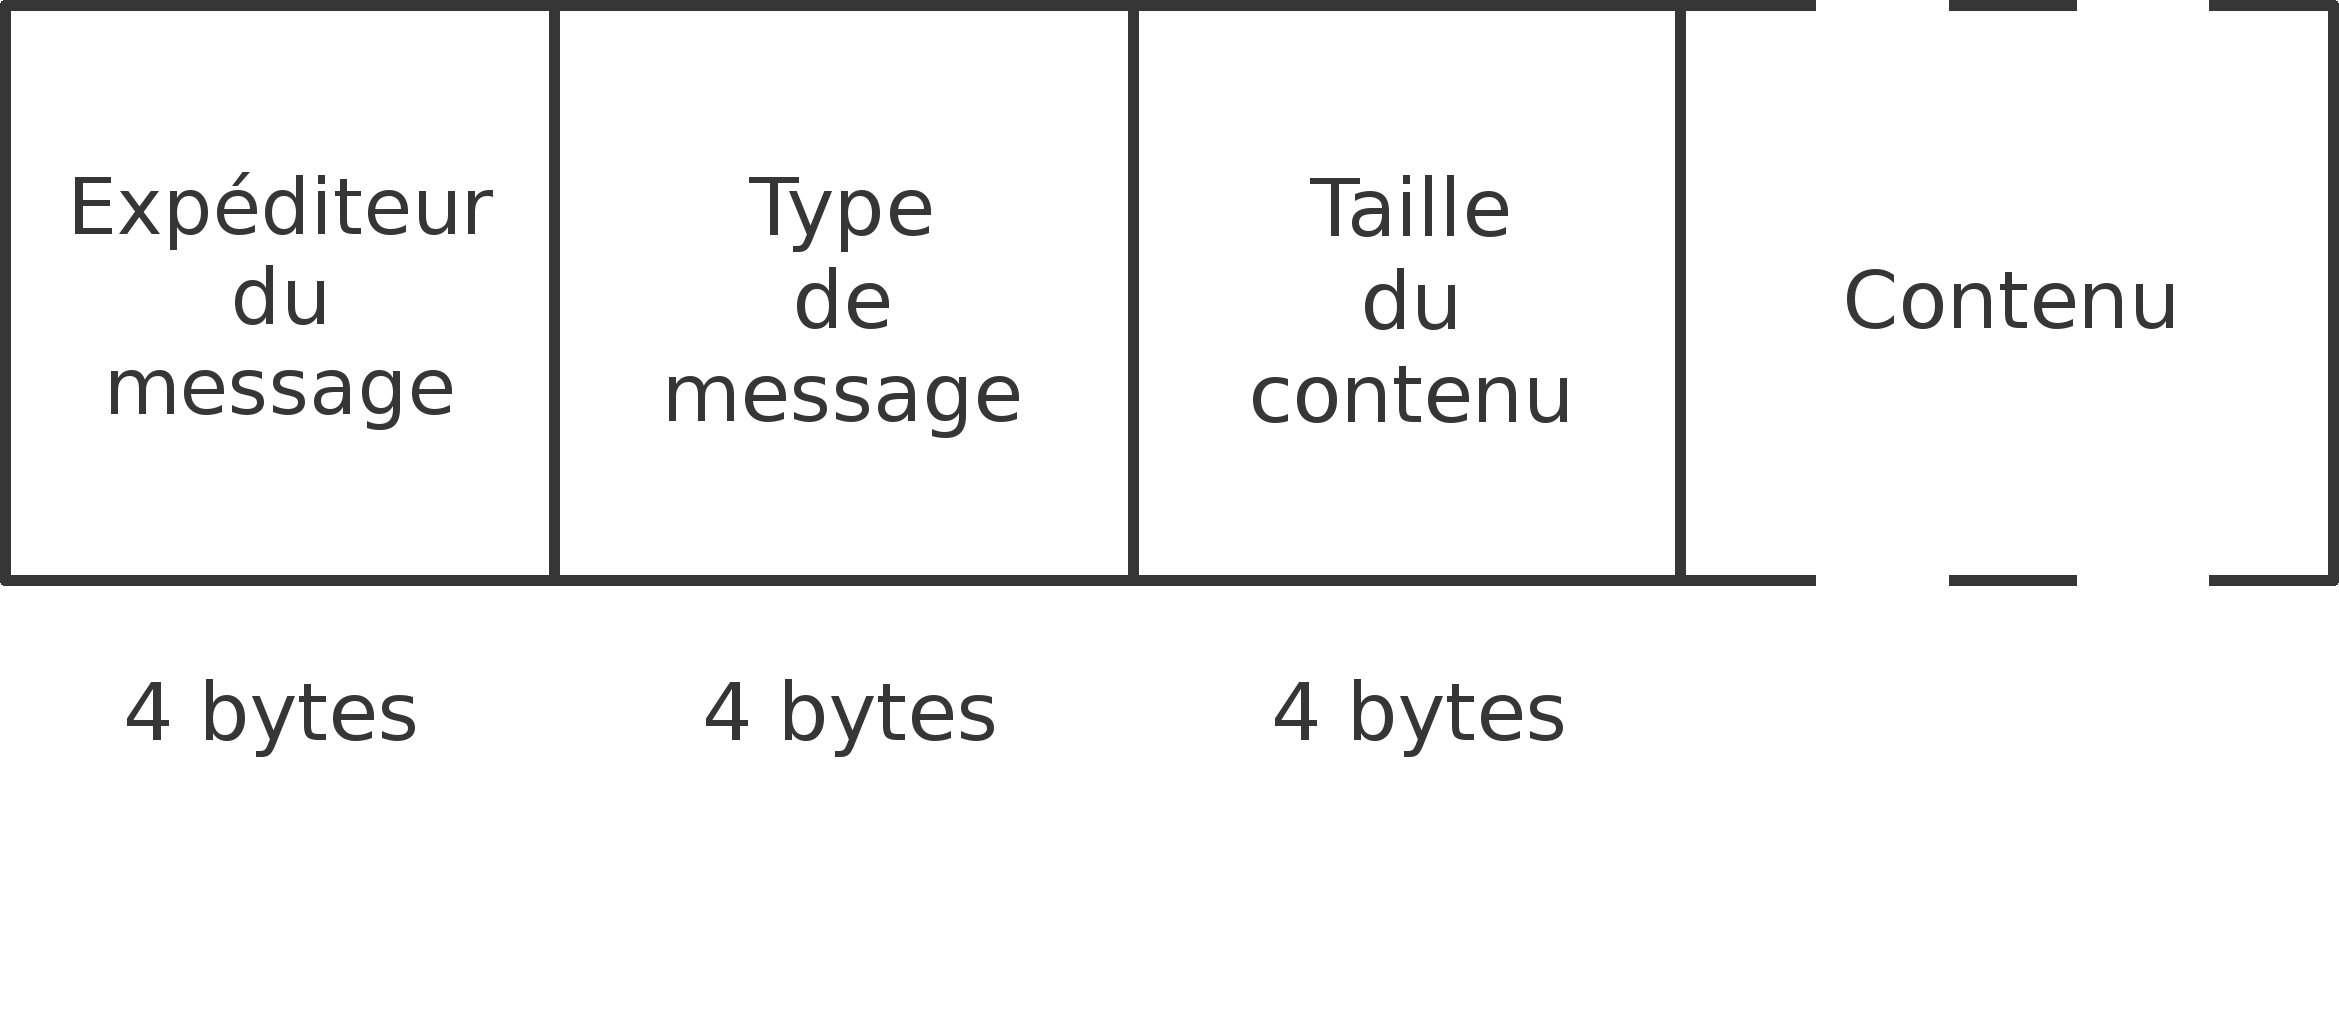
\includegraphics[scale=0.5]{message.png}

\paragraph{}Les messages sont donc constitués de quatre parties : 
\begin{itemize}
\item[1] L'adresse du destinataire, sur 4 octets.
\item[2] Le type de la commande, sur 4 octets également.
\item[3] La taille du contenu du message stocké sur 4 octets.
\item[4] Enfin, le contenu du message.
\end{itemize}

\paragraph{}\textit{Du point de programmation les messages sont stocké dans des byte[] et non pas de char[], car en Java un char est stocké sur 2 octets au lieu de 1. Pour des raisons de compatibilité avec d'autres langages nous avons donc pris la précaution de stocker les caractères des messages transmis sur des octets.}

\paragraph{}Le format ainsi construit des message nous permet donc aisément de savoir qui à envoyé le message et donc de lui répondre, d'envoyer des informations au client ou au serveur. Cela permet aussi au serveur d'envoyer des ordres aux clients (Le serveur peut indiquer à tout les clients que c'est au tour de tel client de prendre le contrôle du dessin), ainsi qu'au client d'envoyer des demandes au serveur (Le client peut demander à prendre la main par exemple).

\subsection{Types de messages échangés.}
\paragraph{}Afin de faire fonctionner notre application nous avons mis en place 13 commandes différentes qui vont être échangées entre les clients et la serveur.

\paragraph{}\begin{itemize}
\item CONNECT : Cette commande est utilisée par le client pour demander une connexion auprès du serveur. Cette commande est utilisée avec comme contenu de message le pseudo désiré par le client. Cette commande attend en retour, comme réponse soit la commande ACCEPT, soit la commande DENY que nous verons plus tard.

\item DISCONNECT : Cette commande est utilisée par le client pour se déconnecter. La commande n'attend rien en retour, le serveur en recevant le message retire le client de sa liste.

\item ACCEPT : Cette commande est envoyé par le serveur au client pour informer que le pseudo demander par le client et valide et que la connexion est accepté. Cette commande est aussi utilisé par le client pour informer le serveur qu'il est près à recevoir le dessin stocké sur le serveur.

\item DENY : Cette commande est envoyé par le serveur dans le cas où le pseudo demander par le client est déjà utilisé. Le client doit alors demander un autre pseudo.

\item  REQUEST$\_$CTRL : Il s'agit de la commande utilisé par les clients pour demander le contrôle du dessin.  Lorsqu'un client demande à prendre le contrôle du dessin le serveur l'ajoute à une liste d'attente, le client en tête de la liste obtient le contrôle pendant 30 secondes. A la fin du temps imparti, le client qui avait le contrôle est éliminé de la liste et on passe au client suivant, le client qui avait le contrôle doit donc redemander le contrôle pour être ré-inséré en fin de liste d'attente.

\item GIVE$\_$CTRL : Cette commande est utilisée par le serveur pour indiquer aux clients, qui prend le contrôle. 

\item LEAVE$\_$CTRL : Cette commande est envoyée du serveur au client qui a la main, afin qu'il la relâche,

\item SUBMIT : Cette commande est envoyé à chaque fois que le dessin est modifié. Le client qui a la main, l'envoie au serveur quand il fait une modification. Le contenu du message joint avec la commande est le contenu du dessin, c'est à dire le document SVG servant à le stocker.

\item UPDATE : Cette commande est renvoyé par le serveur à tous les client après qu'il ait reçu une modification du dessin de la part du client qui a le contrôle du dessin. Comme pour la commande SUBMIT, le contenu du message est le document SVG qui stocke le dessin.
On envoie également cette commande lorsque le client se connecte et qu'il a indiqué avec la commande ACCEPT, qu'il était près à recevoir le dessin.

\item GET$\_$USERS : Les clients utilisent cette commande pour demander la liste des utilisateurs connectés. Nous n'utilisons actuellement pas cette commande dans notre application, mais elle pourrait très bien servir pour afficher la liste complète des utilisateurs à chaque client et pourrait permettre d'ajouter un tchat à notre application de dessin.

\item LIST$\_$USERS : La commande devait servir de réponse à GET$\_$USERS, le contenu du message contient la liste des utilisateurs dans la même room que le client qui reçoit le message.

\item LIST$\_$ROOMS : Cette commande est envoyée par le serveur au client demandant une connexion afin qu'il puisse choisir une room dans la liste. Une room représentant un serveur avec un dessin différent stocké sur chaque room.
Nous n'avons cependant pas eu le temps d'implémenter complètement cette fonctionnalité à notre application, nous n'utilisons donc qu'une seule et unique room.

\item JOIN$\_$ROOM : Cette commande est utilisé par le client pour indiquer au serveur quelle room il veut rejoindre, et donc sur quel dessin il veut travailler.
\end{itemize}

\subsection{Déroulement du protocole}
\paragraph{}Nous allons maintenant suivre dans cette partie le déroulement du protocole depuis la connexion d'un client jusqu'à la modification du dessin et les répercutions de cette modification sur les autres clients.

\paragraph{}Ce protocole peut se diviser en 3 phases : 
\begin{itemize}
	\item[1] La connexion proprement dite, où le client choisit son pseudonyme (ainsi que sa room si cette fonctionnalité est implémentée
	\item[2] La communication de données, que l'on peut séparer en 2 catégories :
	\begin{itemize}
		\item[a] La réception de données, pour tous les clients
		\item[b] L'envoi de mises à jours concernant le dessin, fait seulement par le client ayant la main
	\end{itemize}
	\item[3] La déconnexion du client, annoncée par un message spécifique
\end{itemize}

\textit{Dans ce chapitre, les messages seront décrits sous la forme [ expéditeur ; type ; contenu ] pour plus de lisibilité}

\subsubsection{Connexion}
On suppose que le client A veut se connecter à un serveur, sur lequel sont déjà les clients B et C.
\begin{itemize}
	\item[1] A envoie une demande de connexion au serveur, du type [ A ; CONNECT ; mon\_pseudo ]
	\item[2] Si le serveur ne comporte aucun client portant ce pseudo, il renvoie [ SERVER ; ACCEPT ; ] \\
	Sinon, il renvoie [ SERVER ; DENY ; ] et le client recommence l'étape 1
	\item[3] Comme le client prend un certain temps (variable selon la machine employée) pour préparer son interface, le serveur attends de lui un message de confirmation [ A ; ACCEPT ; ], qui indiquera que la transmission des données de dessin peut commencer
\end{itemize}

\paragraph{}Lorsqu'un client démarre l'application, il se trouve face à une boite de dialogue lui demandant le pseudo qu'il veut utiliser, ainsi que l'adresse du serveur. On ouvre alors une connexion entre le serveur et le client en premier lieu.

Ensuite on test si le pseudo demandé par le client est valide, ceci ce fait en envoyant un message avec la commande CONNECT et le pseudo désiré par le client au serveur. Le serveur test alors l'unicité du pseudonyme, et renvoie le message approprié.

La connexion entre le serveur et le client étant engagé avant même que le client est réellement démarré l'application de dessin, si le client s'arrête (en fermant la fenêtre de connexion) alors le message DISCONNECT est envoyé au serveur qui s'occupe de rompre la connexion.


\paragraph{} Le serveur se met ensuite en attente d'un message du client l'informant qu'il est prêt à recevoir le dessin, l'application pouvant mettre du temps à charger nous devons être sur que tout soit en place pour recevoir et afficher le dessin.

Quand le client à chargé tout ses composants il envoie au serveur le message avec la commande ACCEPT, celui si répond alors en envoyant un message avec la commande UPDATE et comme contenu le dessin SVG qu'il stocke à ce moment. Le client est maintenant correctement connecté et peut alors afficher le dessin, et recevoir les futurs modifications ou demander à prendre la main, etc

\subsubsection{Processus de prise de main}
Afin de pouvoir modifier le dessin, le client A doit avoir la main sur son serveur. Pour cela, il va la demander en envoyant un message [ A ; REQUEST\_CTRL ; ].

\paragraph{} Le serveur recevra cette requête et ajoutera donc A à la fin de la file d'attente pour la prise de main (ou lui donnera la main immédiatement si la file est vide). Lorsque le client ayant la main la rend, le client suivant est pris dans la file d'attente, et reçoit la main pour un temps défini (ici, 30 secondes). Le serveur fait alors savoir au client A que celui-ci a la main par le message [ SERVER ; GIVE\_CTRL ; A ]. Ce message est aussi transmis à tous les autres clients afin que ceux-ci sachent qui a la main.

\paragraph{} Après 30 secondes, le serveur fait savoir au client A que son temps est écoulé, et fait savoir par la même occasion aux autres clients que A n'a plus la main par le message [ SERVER ; LEAVE\_CTRL ; A ].

\subsubsection{Envoi de données par le clients ayant la main}
Lorsque le client A a la main, il va donc renvoyer la totalité du dessin à chaque modification effectuée (souris relachée pour la création de forme, bouton cliqué pour le redimensionnement/déplacement). Bien que ce soit plus coûteux, cette technique permet d'éviter beaucoup de bugs de synchronisation entre le client et le serveur. Ces messages se présenteront sous la forme [ A ; SUBMIT ; nouveau\_dessin ]

\subsubsection{Transmission de l'image du serveur au client}
Le serveur va ensuite transmettre l'image mise à jour à tous les clients (c'est aussi par ce procédé que le client reçoit l'image après sa connexion). De la même façon, pour éviter des problèmes de synchronisation, le dessin est transmis en entier à chaque fois. Le message sera [ SERVER ; UPDATE ; nouveau\_dessin ].

\subsubsection{Déconnexion}
Lorsque le client A souhaite se déconnecter, il prévient d'abord le serveur par un message [ A ; DISCONNECT ; ], pour éviter que le serveur continue d'écouter sur un socket \og vide \fg. Il peut ensuite se déconnecter sans risque : en effet, l'emploi du protocole TCP pour acheminer les messages permet d'être sûr que le serveur a bien reçu cette annonce de déconnexion.

\subsection{Branchement Interface et Réseau}


\section{Recette}

Les test unitaires n'\'etant pas enseign\'es dans notre formation, il s'agissait en premier lieu de se documenter \`a propos de JUnit. Nous avons r\'ealis\'e des tests sur quelques fonctions n'intervenant pas dans l'interface graphique. En effet, les tests unitaires d'\'el\'ements graphiques n\'ecessitent une appr\'ehension plus compl\`ete de JUnit. Le temps manquant, nous n'avons compos\'e des tests que pour la classe Client de l'interface et quelques autres classes de la partie serveur. Finalement, r\'ealiser ces quelques tests nous ont permis d'\'eviter les r\'egressions de code, c'est-\`a-dire \'eviter qu'une modification ou une am\'elioration d'une ou plusieurs fonctions ne r\'epondent plus \`a tous les cas d'utilisation. 

\section{Gestion de projet}
Au fil de la réalisation de ce projet, il nous est apparu que la gestion de projet a été d'une importance capitale. En effet, si nous avions lu le cahier des charges chacun de notre côté, sans nous soucier de la répartition des tâches, des délais à tenir et de la cohérence entre nous, il est plus que probable que le projet n'aurait pas été terminé dans les temps. Nous expliquerons dans cette partie les différentes techniques de gestion de projet mises en places ainsi que les problèmes rencontrés.

\subsection{Réunion}
Notre projet a été ponctué au fil de temps d'un certain nombre de réunion, chacune ayant des objectifs différents.

\paragraph{} Notre projet a débuté par une première réunion durant laquelle nous avons lu et analyser le cahier des charges. C'est durant celle-ci que nous nous sommes mis d'accord sur les outils et solutions que nous utiliserions, que nous avons défini de manière grossière l'architecture utilisée et organisé la suite du projet. Nous avons notamment dû choisir un chef de projet dont la fonction serait d'organiser et de planifier le projet afin de le mener à sa bonne réalisation mais aussi d'être le contact privilégié avec les enseignants. Parmi nous, Romain et Jean-Baptiste se sont portés volontaire pour cette fonction. Finalement, après s'être mis d'accord, c'est Jean-Baptiste qui a pris cette fonction.

\paragraph{} Contrairement à des projets d'envergure dont la gestion de projet demande un investissement en temps conséquent, la gestion de notre projet a tout de même permis au chef de projet de participer activement au développement et aux développeurs de donner souvent leur avis quant à la gestion de projet.

\paragraph{} Comme cela est visible dans le planning, nous avons ensuite ponctuer la période dédiée au projet de différentes réunions de suivi, qui avaient pour but de vérifier l'avancement du projet, de prévoir d’éventuels problèmes pouvant modifier le planning. Il s'est avéré que ces réunions avaient plutôt pour but de vérifier l'avancement du projet et d'effectuer les modifications du planning suivant les tâches réalisés et à venir. Cet état de fait fut possible grâce à notre proximité, ce qui nous a permis de parler des différents problèmes rencontrés ainsi que des solutions à apporter au fil de l'eau et non pendant les réunions ponctuelles.

\paragraph{} A mi-parcourt, nous avons dû réaliser une réunion avec M Richer de manière à expliquer à quel point en était notre projet. Nous avons donc préparé cette réunion entre nous en faisant un bilan sur les fonctionnalités terminées, les fonctionnalités en cours et les fonctionnalités qui n'étaient pas commencées ainsi qu'en mettant par écrit les différents points à éclaircir de manière à répondre le mieux possibles au cahier des charges.

\subsection{Planning}
De manière à terminer le projet dans le temps imparti tout en livrant toutes les fonctionnalités, nous avons mis en place un planning résumant chaque tâche avec une estimation de la durée de chacune.

\paragraph{} Ce planning s'est majoritairement appuyé sur le chiffrage effectué précédemment et a donc évolué au fil du temps, certaines tâches se révélant plus rapide alors que d'autres furent plus longue à réaliser. Nous avons donc mis à jours ce planning de manière à savoir l'avancement de chacun et les tâches suivantes à réaliser.

\paragraph{} Le planning a été réaliser grâce à Gantt Project. Le planning ainsi créé étant trop imposant pour être inséré dans le rapport, il est trouvable sous forme d'image dans l'archive contenant le projet (cf : Dessin collaboratif – Planning). Le diagramme de PERT quant à lui été généré grâce à Gantt Project à partir du planning (cf : Dessin collaboratif – Diagramme de PERT).

\section{Bilan}
\subsection{Bilan technique}
Ce projet a été très formateur pour chacun d'entre nous et ce pour divers raisons. 

\paragraph{} En premier lieu, il nous a permis d'améliorer notre maîtrise du langage Java. En effet, venant chacun de formations différentes, nous ne sommes pas partis avec la même maîtrise de ce langage et, bien que nous connaissions tous des langages objets, il a fallut que nous nous mettions au même niveau.

\paragraph{} Ensuite, nous avons découvert différents outils nécessaires à la bonne mises en œuvre de ce projet. Bien que nous en connaissions déjà certains comme Git et Swing, ce projet nous a permis d'approfondir nos connaissances et d'être plus efficace et rapide à les utiliser. Mais nous avons aussi eu l'occasion de découvrir d'autres outils et bibliothèques que nous n'aurions peut-être pas découvert sans ce projet comme Batik par exemple.

\paragraph{} Mais ce projet nous a surtout montré que le choix des outils en début de projet est déterminant dans la bonne mise en œuvre ce projet et qu'un mauvais choix d'outils est déterminant par la suite. Dans notre cas, nous avons compris que, même si Batik permet de gérer simplement l'affichage de .svg, cette bibliothèque permet des traitements génériques mais ne répondant pas forcément à nos besoins. Notamment, nous avons besoin de ré-afficher le canvas contenant l'image, mais la bibliothèque ne gère pas le double buffering, cause du clignotement de l'image lors des modifications. Nous en avons conclu que, si nous avions à refaire ce projet, nous n'utiliserions pas cette bibliothèque, préférant créer nos propres composants répondant au problème plutôt que de tenter de modifier les comportement de Batik, de peur de la rendre instable.

\subsection{Bilan humain}
Ce projet nous a beaucoup appris, notamment concernant la gestion de projet. En effet, beaucoup des processus mis en œuvre afin de mener à bien notre projet peuvent finalement s'apparenter à ceux utilisés en entreprise. En effet, notre chiffrage, bien que sommaire permettra en entreprise d'estimer combien de temps de développement demandera un projet. Le planning quant à lui est similaire et permet aux développeurs de connaître leurs affectations au fil du temps.

\section*{Conclusion}

\section*{Lexique}

\section*{Annexe}

\end{document}